\documentclass{beamer}
\usepackage[english,russian]{babel}
\usepackage[utf8]{inputenc}
\usetheme{Singapore} %Goettingen,  Montpellier, Singapore

% \usetheme[pageofpages=of,% String used between the current page and the
%                          % total page count.
%           bullet=circle,% Use circles instead of squares for bullets.
%           titleline=true,% Show a line below the frame title.
%           alternativetitlepage=true,% Use the fancy title page.
%           titlepagelogo= msu, %logo-polito,% Logo for the first page.
%           %watermark=msu,%watermark-polito,% Watermark used in every page.
%           %watermarkheight=100px,% Height of the watermark.
%           %watermarkheightmult=2,% The watermark image is 4 times bigger
%                                 % than watermarkheight.
%           ]{Torino}
\usepackage{verbatim}
\usepackage{listings}

\usepackage{tikz}
\usetikzlibrary{shapes,arrows}

\usetikzlibrary{shapes.geometric,shapes.arrows,decorations.pathmorphing}
\usetikzlibrary{matrix,chains,scopes,positioning,arrows,fit,arrows,backgrounds}
\tikzstyle{block} = [rectangle, draw,  text width=20em, text centered, minimum height=4em, top color=white,
    bottom color=blue!50!black!20, draw=blue!40!black!60, very
    thick, rounded corners]
\tikzstyle{de} = [diamond, drawshade, top color=white,
    bottom color=blue!50!black!20, draw=blue!40!black!60, very
    thick, text centered, rounded corners, text width=6em, text badly centered, node distance=3cm, inner sep=0pt]

%     text width=5em, text centered, rounded corners, minimum height=4em]
 \tikzstyle{decision} = [diamond, drawshade,  top color=white,
    bottom color=blue!50!black!20, draw=blue!40!black!60, very
    thick, text width=4.5em, text badly centered, node distance=3cm, inner sep=0pt]

 

\tikzstyle{line} = [draw, -latex']
\tikzstyle{cloud} = [draw, ellipse,fill=red!20, node distance=3cm,
    minimum height=2em]
   
\tikzset{blue dotted/.style={draw=blue!50!white, line width=1pt,
                               dash pattern=on 1pt off 4pt on 6pt off 4pt,
                                inner sep=4mm, rectangle, rounded corners}}
\tikzstyle{blockwhite} = [rectangle, draw,  text width=5em, text centered, minimum height=4em, draw=white, fill=white]
\tikzstyle{bl} = [block, shade, top color=white,
    bottom color=blue!50!black!20, draw=blue!40!black!60, very
    thick, text width=20em, text centered, rounded corners, minimum height=4em]
\tikzstyle{blk} = [block, shade, top color=white,
    bottom color=blue!50!black!20, draw=blue!40!black!60, very
    thick, text width=9em, text centered, rounded corners, minimum height=4em]
\tikzstyle{blkred}=[blk, bottom color=red!50!black!20]
\tikzstyle{blkyell}=[blk, bottom color=yellow!50!black!20]
\tikzstyle{blb} = [block, shade, top color=white,
    bottom color=blue!50!black!20, draw=blue!40!black!60, very
    thick, text width=10em, text centered, rounded corners, minimum height=4em]

\def\watermarkoff{\def\beamer@decolines@watermark{}}
%\setbeamercolor{alert text}{fg=green}

\usepackage{wrapfig}
\begin{document}
\title{Интеграция средств гранулярного контроля безопасности поведения
        приложений в ОС Линукс}  
\author{\small{Фёдор Сахаров}\\ \small{\href{mailto:sakharov@lvk.cs.msu.su}{sakharov@lvk.cs.msu.su}}}
\institute{Лаборатория вычислительных комплексов ВМК \\ МГУ имени М.В.Ломоносова}
\date{Москва, 2011} 
\begin{frame}[t, plain] 
\watermarkoff
 \titlepage
\end{frame}

\begin{frame}{Краткое содержание лекции}
\watermarkoff
\begin{block}{Сегодня в планах:}
 \begin{itemize}
  \item Стандартная модель безопасности в UNIX-подобных системах
  \item Расширения стандартной модельи безопасности.
  \item SELinux: motivation
  \item SELinux: theory
  \item SELinux: practice
  \item SELinux: hit the fan
 \end{itemize}
\end{block}
\end{frame}

\begin{frame}[fragile]{Стандартная модель безопасности в UNIX}
Основная идея~--- система привилегий.
\bigskip

В системе существует набор пользователей.
\bigskip
\begin{lstlisting}
# cat /etc/passwd | sed 's/:.*//g'
root
bin
daemon
adm
...
\end{lstlisting}

Множество пользователей разбивается на подмножества,
называемые группами.
\end{frame}


\begin{frame}[fragile]{Стандартная модель безопасности в UNIX}
В системе существует множество файлов.
У каждого файла есть владелец(один из пользователей)
и группа владельцев.

\bigskip
С каждым из файлов ассоциирован набор прав доступа.

\begin{block}{Набор прав включает в себя:}
\begin{itemize}
\item Права владельца
\item Права группы владельцев
\item Права остальных пользователей
\end{itemize}
\end{block}

\begin{lstlisting}
-rw-r--r-- 1 root root /etc/passwd
\end{lstlisting}

\end{frame}

\begin{frame}[fragile]{Стандартная модель безопасности в UNIX}
\bfseries{Любой процесс, запущенный пользователем, обладает всеми правами этого пользователя.}

\begin{center}
\scalebox{.60}{
    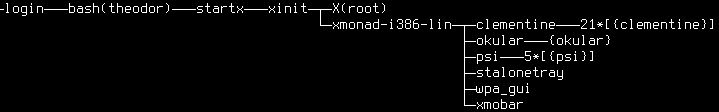
\includegraphics{pstree.png}
}
\end{center}
\end{frame}

\begin{frame}[fragile]{Стандартная модель безопасности в UNIX}
\bfseries{Любой процесс, запущенный пользователем, обладает всеми правами этого пользователя.}

\begin{block}{Это значит, что:}

\begin{itemize}
\item Права процессов ограничены правами пользователя и это хорошо.
        Позволяет во многих случаях
        сохранить конфиденциальность и целостность информации.

\item Права процессов ограничены правами пользователя и это плохо.
        Набор привилегий пользователя, как правило, является слишком
        широким для любого из процессов, запущенных данным пользователем.

\end{itemize}
\end{block}

\end{frame}

\begin{frame}[fragile]{Стандартная мдоель безопасности в UNIX}
Набор привилегий пользователя, как правило, является слишком
широким для любого из процессов, запущенных данным пользователем.

\bigskip

Любое приложение имеет доступ к любым ресурсам, к которым имеет доступ
пользователь.

\bigskip

Например, skype имеет право на доступ к файлам в ~/.mozilla/firefox.

\end{frame}

\begin{frame}[fragile]{Стандартная модель безопасности в UNIX}
Набор привилегий пользователя, как правило, является слишком
широким для любого из процессов, запущенных данным пользователем.

\bigskip

В результате, компрометация любого из пользовательских приложений
позволяет злоумышленнику получить все привилегии пользователя.
\begin{center}
\scalebox{.65}{
    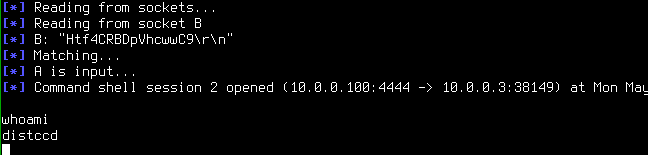
\includegraphics{whoami.png}
}
\end{center}
\end{frame}

\begin{frame}[fragile]{Стандартная модель безопасности в UNIX}
С точки зрения \href{http://en.wikipedia.org/wiki/Common\_Criteria}{<<Общих Критериев>> (Common Criteria)}
в стандартной модели безопасноти UNIX существует большой потенциал для повсеместных
улучшений.

\begin{block}{В частности, могут быть реализованы расширения:}
\begin{itemize}
\item Role Based Access Control
\item Mandatory Access Control
\item etc.
\end{itemize}
\end{block}

\end{frame}

\begin{frame}[fragile]{Расширения стандартной модели безопасности}

В результате попыток расширить стандартную систему безопасности UNIX
появилось множество проектов.

\begin{block}{В разное время разными людьми были сделаны:}

\begin{itemize}
\item SELinux (\href{http://selinuxproject.org}{selinuxproject.org})
\item AppArmor (\href{http://wiki.apparmor.net/index.php/Main\_Page}{apparmor.net})
\item Tomoyo Linux (\href{http://tomoyo.sourceforge.jp/}{tomoyo.sourceforge.jp})
\item GRSecurity (\href{http://grsecurity.net/}{grsecurity.net})
\item TrustedBSD, SEBSD, SEDarwin, Darwin Seatbelt
\end{itemize}
\end{block}

\end{frame}

\begin{frame}{SELinux}
Далее речь пойдет о системе 
SELinux (Security Enhanced Linux)~--- проект реализованный в
NSA и вошедший в ядро Linux.

\begin{block}{SELinux реализует следующие модели безопасности:}

\begin{itemize}
\item Mandatory Access Control, представленный двумя типами:
    \begin{itemize}
    \item Type Enforcement (TE)
    \item Multi-Level Security (MLS)
    \end{itemize}
\item Role Based Acces Control
\end{itemize}

\end{block}

\end{frame}

\begin{frame}{Спасибо за внимание. Вопросы?}
\begin{center}
\LARGE{Спасибо за внимание. Вопросы?}
\end{center}

   
\end{frame}

\end{document}


